% Created by tikzDevice version 0.12.6 on 2024-01-22 00:12:43
% !TEX encoding = UTF-8 Unicode
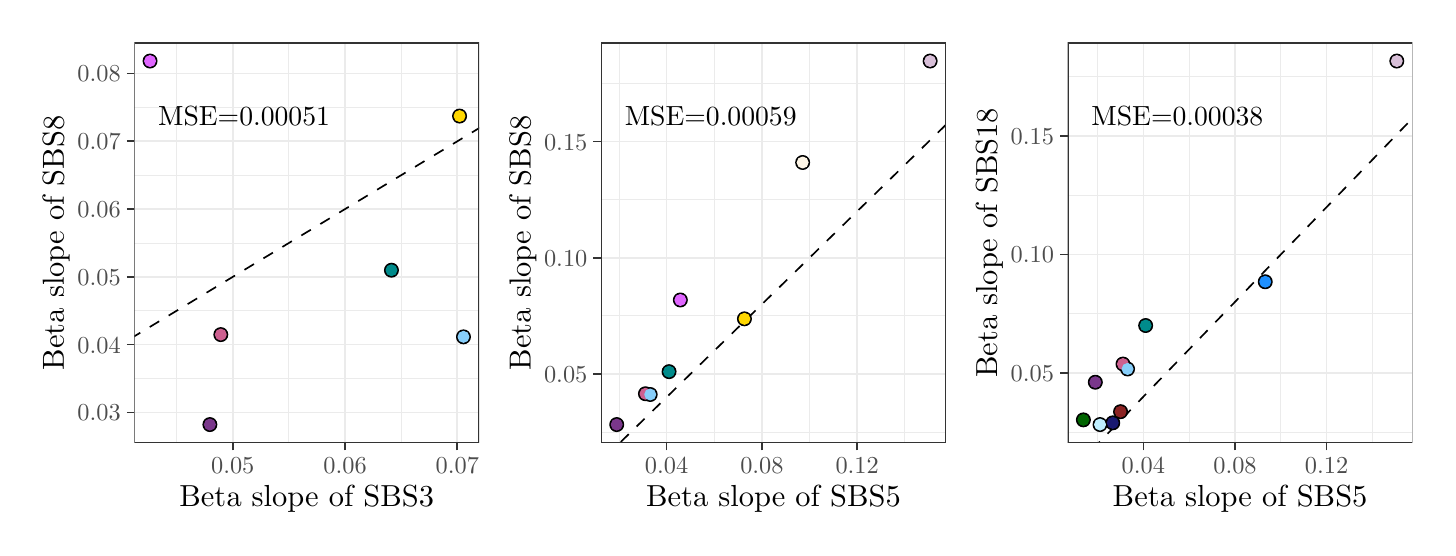
\begin{tikzpicture}[x=1pt,y=1pt]
\definecolor{fillColor}{RGB}{255,255,255}
\path[use as bounding box,fill=fillColor,fill opacity=0.00] (0,0) rectangle (505.89,180.67);
\begin{scope}
\path[clip] (  0.00,  0.00) rectangle (168.63,180.67);
\definecolor{drawColor}{RGB}{255,255,255}
\definecolor{fillColor}{RGB}{255,255,255}

\path[draw=drawColor,line width= 0.6pt,line join=round,line cap=round,fill=fillColor] (  0.00,  0.00) rectangle (168.63,180.68);
\end{scope}
\begin{scope}
\path[clip] ( 38.56, 30.69) rectangle (163.13,175.17);
\definecolor{fillColor}{RGB}{255,255,255}

\path[fill=fillColor] ( 38.56, 30.69) rectangle (163.13,175.17);
\definecolor{drawColor}{gray}{0.92}

\path[draw=drawColor,line width= 0.3pt,line join=round] ( 38.56, 53.88) --
	(163.13, 53.88);

\path[draw=drawColor,line width= 0.3pt,line join=round] ( 38.56, 78.37) --
	(163.13, 78.37);

\path[draw=drawColor,line width= 0.3pt,line join=round] ( 38.56,102.87) --
	(163.13,102.87);

\path[draw=drawColor,line width= 0.3pt,line join=round] ( 38.56,127.36) --
	(163.13,127.36);

\path[draw=drawColor,line width= 0.3pt,line join=round] ( 38.56,151.85) --
	(163.13,151.85);

\path[draw=drawColor,line width= 0.3pt,line join=round] ( 53.83, 30.69) --
	( 53.83,175.17);

\path[draw=drawColor,line width= 0.3pt,line join=round] ( 94.39, 30.69) --
	( 94.39,175.17);

\path[draw=drawColor,line width= 0.3pt,line join=round] (134.96, 30.69) --
	(134.96,175.17);

\path[draw=drawColor,line width= 0.6pt,line join=round] ( 38.56, 41.63) --
	(163.13, 41.63);

\path[draw=drawColor,line width= 0.6pt,line join=round] ( 38.56, 66.13) --
	(163.13, 66.13);

\path[draw=drawColor,line width= 0.6pt,line join=round] ( 38.56, 90.62) --
	(163.13, 90.62);

\path[draw=drawColor,line width= 0.6pt,line join=round] ( 38.56,115.11) --
	(163.13,115.11);

\path[draw=drawColor,line width= 0.6pt,line join=round] ( 38.56,139.61) --
	(163.13,139.61);

\path[draw=drawColor,line width= 0.6pt,line join=round] ( 38.56,164.10) --
	(163.13,164.10);

\path[draw=drawColor,line width= 0.6pt,line join=round] ( 74.11, 30.69) --
	( 74.11,175.17);

\path[draw=drawColor,line width= 0.6pt,line join=round] (114.68, 30.69) --
	(114.68,175.17);

\path[draw=drawColor,line width= 0.6pt,line join=round] (155.24, 30.69) --
	(155.24,175.17);
\definecolor{drawColor}{RGB}{0,0,0}

\path[draw=drawColor,line width= 0.6pt,dash pattern=on 4pt off 4pt ,line join=round] (-86.02, -6.06) -- (287.70,219.58);
\definecolor{fillColor}{RGB}{0,0,0}

\path[draw=drawColor,line width= 0.4pt,line join=round,line cap=round,fill=fillColor] (156.06,148.73) circle (  2.50);

\path[draw=drawColor,line width= 0.4pt,line join=round,line cap=round,fill=fillColor] ( 69.79, 69.76) circle (  2.50);

\path[draw=drawColor,line width= 0.4pt,line join=round,line cap=round,fill=fillColor] (131.45, 93.03) circle (  2.50);

\path[draw=drawColor,line width= 0.4pt,line join=round,line cap=round,fill=fillColor] ( 65.84, 37.25) circle (  2.50);

\path[draw=drawColor,line width= 0.4pt,line join=round,line cap=round,fill=fillColor] ( 44.22,168.61) circle (  2.50);

\path[draw=drawColor,line width= 0.4pt,line join=round,line cap=round,fill=fillColor] (157.47, 68.95) circle (  2.50);
\definecolor{drawColor}{RGB}{255,215,0}
\definecolor{fillColor}{RGB}{255,215,0}

\path[draw=drawColor,line width= 0.4pt,line join=round,line cap=round,fill=fillColor] (156.06,148.73) circle (  1.96);
\definecolor{drawColor}{RGB}{205,96,144}
\definecolor{fillColor}{RGB}{205,96,144}

\path[draw=drawColor,line width= 0.4pt,line join=round,line cap=round,fill=fillColor] ( 69.79, 69.76) circle (  1.96);
\definecolor{drawColor}{RGB}{0,139,139}
\definecolor{fillColor}{RGB}{0,139,139}

\path[draw=drawColor,line width= 0.4pt,line join=round,line cap=round,fill=fillColor] (131.45, 93.03) circle (  1.96);
\definecolor{drawColor}{RGB}{122,55,139}
\definecolor{fillColor}{RGB}{122,55,139}

\path[draw=drawColor,line width= 0.4pt,line join=round,line cap=round,fill=fillColor] ( 65.84, 37.25) circle (  1.96);
\definecolor{drawColor}{RGB}{224,102,255}
\definecolor{fillColor}{RGB}{224,102,255}

\path[draw=drawColor,line width= 0.4pt,line join=round,line cap=round,fill=fillColor] ( 44.22,168.61) circle (  1.96);
\definecolor{drawColor}{RGB}{135,206,250}
\definecolor{fillColor}{RGB}{135,206,250}

\path[draw=drawColor,line width= 0.4pt,line join=round,line cap=round,fill=fillColor] (157.47, 68.95) circle (  1.96);
\definecolor{drawColor}{RGB}{0,0,0}

\node[text=drawColor,anchor=base,inner sep=0pt, outer sep=0pt, scale=  1.00] at ( 78.19,145.48) {MSE=0.00051};
\definecolor{drawColor}{gray}{0.20}

\path[draw=drawColor,line width= 0.6pt,line join=round,line cap=round] ( 38.56, 30.69) rectangle (163.13,175.17);
\end{scope}
\begin{scope}
\path[clip] (  0.00,  0.00) rectangle (505.89,180.67);
\definecolor{drawColor}{gray}{0.30}

\node[text=drawColor,anchor=base east,inner sep=0pt, outer sep=0pt, scale=  0.88] at ( 33.61, 38.60) {0.03};

\node[text=drawColor,anchor=base east,inner sep=0pt, outer sep=0pt, scale=  0.88] at ( 33.61, 63.10) {0.04};

\node[text=drawColor,anchor=base east,inner sep=0pt, outer sep=0pt, scale=  0.88] at ( 33.61, 87.59) {0.05};

\node[text=drawColor,anchor=base east,inner sep=0pt, outer sep=0pt, scale=  0.88] at ( 33.61,112.08) {0.06};

\node[text=drawColor,anchor=base east,inner sep=0pt, outer sep=0pt, scale=  0.88] at ( 33.61,136.58) {0.07};

\node[text=drawColor,anchor=base east,inner sep=0pt, outer sep=0pt, scale=  0.88] at ( 33.61,161.07) {0.08};
\end{scope}
\begin{scope}
\path[clip] (  0.00,  0.00) rectangle (505.89,180.67);
\definecolor{drawColor}{gray}{0.20}

\path[draw=drawColor,line width= 0.6pt,line join=round] ( 35.81, 41.63) --
	( 38.56, 41.63);

\path[draw=drawColor,line width= 0.6pt,line join=round] ( 35.81, 66.13) --
	( 38.56, 66.13);

\path[draw=drawColor,line width= 0.6pt,line join=round] ( 35.81, 90.62) --
	( 38.56, 90.62);

\path[draw=drawColor,line width= 0.6pt,line join=round] ( 35.81,115.11) --
	( 38.56,115.11);

\path[draw=drawColor,line width= 0.6pt,line join=round] ( 35.81,139.61) --
	( 38.56,139.61);

\path[draw=drawColor,line width= 0.6pt,line join=round] ( 35.81,164.10) --
	( 38.56,164.10);
\end{scope}
\begin{scope}
\path[clip] (  0.00,  0.00) rectangle (505.89,180.67);
\definecolor{drawColor}{gray}{0.20}

\path[draw=drawColor,line width= 0.6pt,line join=round] ( 74.11, 27.94) --
	( 74.11, 30.69);

\path[draw=drawColor,line width= 0.6pt,line join=round] (114.68, 27.94) --
	(114.68, 30.69);

\path[draw=drawColor,line width= 0.6pt,line join=round] (155.24, 27.94) --
	(155.24, 30.69);
\end{scope}
\begin{scope}
\path[clip] (  0.00,  0.00) rectangle (505.89,180.67);
\definecolor{drawColor}{gray}{0.30}

\node[text=drawColor,anchor=base,inner sep=0pt, outer sep=0pt, scale=  0.88] at ( 74.11, 19.68) {0.05};

\node[text=drawColor,anchor=base,inner sep=0pt, outer sep=0pt, scale=  0.88] at (114.68, 19.68) {0.06};

\node[text=drawColor,anchor=base,inner sep=0pt, outer sep=0pt, scale=  0.88] at (155.24, 19.68) {0.07};
\end{scope}
\begin{scope}
\path[clip] (  0.00,  0.00) rectangle (505.89,180.67);
\definecolor{drawColor}{RGB}{0,0,0}

\node[text=drawColor,anchor=base,inner sep=0pt, outer sep=0pt, scale=  1.10] at (100.84,  7.64) {Beta slope of SBS3};
\end{scope}
\begin{scope}
\path[clip] (  0.00,  0.00) rectangle (505.89,180.67);
\definecolor{drawColor}{RGB}{0,0,0}

\node[text=drawColor,rotate= 90.00,anchor=base,inner sep=0pt, outer sep=0pt, scale=  1.10] at ( 13.08,102.93) {Beta slope of SBS8};
\end{scope}
\begin{scope}
\path[clip] (168.63,  0.00) rectangle (337.26,180.67);
\definecolor{drawColor}{RGB}{255,255,255}
\definecolor{fillColor}{RGB}{255,255,255}

\path[draw=drawColor,line width= 0.6pt,line join=round,line cap=round,fill=fillColor] (168.63,  0.00) rectangle (337.26,180.68);
\end{scope}
\begin{scope}
\path[clip] (207.19, 30.69) rectangle (331.76,175.17);
\definecolor{fillColor}{RGB}{255,255,255}

\path[fill=fillColor] (207.19, 30.69) rectangle (331.76,175.17);
\definecolor{drawColor}{gray}{0.92}

\path[draw=drawColor,line width= 0.3pt,line join=round] (207.19, 34.56) --
	(331.76, 34.56);

\path[draw=drawColor,line width= 0.3pt,line join=round] (207.19, 76.53) --
	(331.76, 76.53);

\path[draw=drawColor,line width= 0.3pt,line join=round] (207.19,118.51) --
	(331.76,118.51);

\path[draw=drawColor,line width= 0.3pt,line join=round] (207.19,160.48) --
	(331.76,160.48);

\path[draw=drawColor,line width= 0.3pt,line join=round] (213.68, 30.69) --
	(213.68,175.17);

\path[draw=drawColor,line width= 0.3pt,line join=round] (248.11, 30.69) --
	(248.11,175.17);

\path[draw=drawColor,line width= 0.3pt,line join=round] (282.53, 30.69) --
	(282.53,175.17);

\path[draw=drawColor,line width= 0.3pt,line join=round] (316.96, 30.69) --
	(316.96,175.17);

\path[draw=drawColor,line width= 0.6pt,line join=round] (207.19, 55.54) --
	(331.76, 55.54);

\path[draw=drawColor,line width= 0.6pt,line join=round] (207.19, 97.52) --
	(331.76, 97.52);

\path[draw=drawColor,line width= 0.6pt,line join=round] (207.19,139.49) --
	(331.76,139.49);

\path[draw=drawColor,line width= 0.6pt,line join=round] (230.89, 30.69) --
	(230.89,175.17);

\path[draw=drawColor,line width= 0.6pt,line join=round] (265.32, 30.69) --
	(265.32,175.17);

\path[draw=drawColor,line width= 0.6pt,line join=round] (299.75, 30.69) --
	(299.75,175.17);
\definecolor{drawColor}{RGB}{0,0,0}

\path[draw=drawColor,line width= 0.6pt,dash pattern=on 4pt off 4pt ,line join=round] ( 82.61,-97.49) -- (456.33,267.05);
\definecolor{fillColor}{RGB}{0,0,0}

\path[draw=drawColor,line width= 0.4pt,line join=round,line cap=round,fill=fillColor] (259.00, 75.46) circle (  2.50);

\path[draw=drawColor,line width= 0.4pt,line join=round,line cap=round,fill=fillColor] (223.23, 48.39) circle (  2.50);

\path[draw=drawColor,line width= 0.4pt,line join=round,line cap=round,fill=fillColor] (326.10,168.61) circle (  2.50);

\path[draw=drawColor,line width= 0.4pt,line join=round,line cap=round,fill=fillColor] (280.03,131.95) circle (  2.50);

\path[draw=drawColor,line width= 0.4pt,line join=round,line cap=round,fill=fillColor] (231.76, 56.37) circle (  2.50);

\path[draw=drawColor,line width= 0.4pt,line join=round,line cap=round,fill=fillColor] (212.85, 37.25) circle (  2.50);

\path[draw=drawColor,line width= 0.4pt,line join=round,line cap=round,fill=fillColor] (235.84, 82.27) circle (  2.50);

\path[draw=drawColor,line width= 0.4pt,line join=round,line cap=round,fill=fillColor] (224.95, 48.12) circle (  2.50);
\definecolor{drawColor}{RGB}{255,215,0}
\definecolor{fillColor}{RGB}{255,215,0}

\path[draw=drawColor,line width= 0.4pt,line join=round,line cap=round,fill=fillColor] (259.00, 75.46) circle (  1.96);
\definecolor{drawColor}{RGB}{205,96,144}
\definecolor{fillColor}{RGB}{205,96,144}

\path[draw=drawColor,line width= 0.4pt,line join=round,line cap=round,fill=fillColor] (223.23, 48.39) circle (  1.96);
\definecolor{drawColor}{RGB}{216,191,216}
\definecolor{fillColor}{RGB}{216,191,216}

\path[draw=drawColor,line width= 0.4pt,line join=round,line cap=round,fill=fillColor] (326.10,168.61) circle (  1.96);
\definecolor{drawColor}{RGB}{253,245,230}
\definecolor{fillColor}{RGB}{253,245,230}

\path[draw=drawColor,line width= 0.4pt,line join=round,line cap=round,fill=fillColor] (280.03,131.95) circle (  1.96);
\definecolor{drawColor}{RGB}{0,139,139}
\definecolor{fillColor}{RGB}{0,139,139}

\path[draw=drawColor,line width= 0.4pt,line join=round,line cap=round,fill=fillColor] (231.76, 56.37) circle (  1.96);
\definecolor{drawColor}{RGB}{122,55,139}
\definecolor{fillColor}{RGB}{122,55,139}

\path[draw=drawColor,line width= 0.4pt,line join=round,line cap=round,fill=fillColor] (212.85, 37.25) circle (  1.96);
\definecolor{drawColor}{RGB}{224,102,255}
\definecolor{fillColor}{RGB}{224,102,255}

\path[draw=drawColor,line width= 0.4pt,line join=round,line cap=round,fill=fillColor] (235.84, 82.27) circle (  1.96);
\definecolor{drawColor}{RGB}{135,206,250}
\definecolor{fillColor}{RGB}{135,206,250}

\path[draw=drawColor,line width= 0.4pt,line join=round,line cap=round,fill=fillColor] (224.95, 48.12) circle (  1.96);
\definecolor{drawColor}{RGB}{0,0,0}

\node[text=drawColor,anchor=base,inner sep=0pt, outer sep=0pt, scale=  1.00] at (246.82,145.48) {MSE=0.00059};
\definecolor{drawColor}{gray}{0.20}

\path[draw=drawColor,line width= 0.6pt,line join=round,line cap=round] (207.19, 30.69) rectangle (331.76,175.17);
\end{scope}
\begin{scope}
\path[clip] (  0.00,  0.00) rectangle (505.89,180.67);
\definecolor{drawColor}{gray}{0.30}

\node[text=drawColor,anchor=base east,inner sep=0pt, outer sep=0pt, scale=  0.88] at (202.24, 52.51) {0.05};

\node[text=drawColor,anchor=base east,inner sep=0pt, outer sep=0pt, scale=  0.88] at (202.24, 94.49) {0.10};

\node[text=drawColor,anchor=base east,inner sep=0pt, outer sep=0pt, scale=  0.88] at (202.24,136.46) {0.15};
\end{scope}
\begin{scope}
\path[clip] (  0.00,  0.00) rectangle (505.89,180.67);
\definecolor{drawColor}{gray}{0.20}

\path[draw=drawColor,line width= 0.6pt,line join=round] (204.44, 55.54) --
	(207.19, 55.54);

\path[draw=drawColor,line width= 0.6pt,line join=round] (204.44, 97.52) --
	(207.19, 97.52);

\path[draw=drawColor,line width= 0.6pt,line join=round] (204.44,139.49) --
	(207.19,139.49);
\end{scope}
\begin{scope}
\path[clip] (  0.00,  0.00) rectangle (505.89,180.67);
\definecolor{drawColor}{gray}{0.20}

\path[draw=drawColor,line width= 0.6pt,line join=round] (230.89, 27.94) --
	(230.89, 30.69);

\path[draw=drawColor,line width= 0.6pt,line join=round] (265.32, 27.94) --
	(265.32, 30.69);

\path[draw=drawColor,line width= 0.6pt,line join=round] (299.75, 27.94) --
	(299.75, 30.69);
\end{scope}
\begin{scope}
\path[clip] (  0.00,  0.00) rectangle (505.89,180.67);
\definecolor{drawColor}{gray}{0.30}

\node[text=drawColor,anchor=base,inner sep=0pt, outer sep=0pt, scale=  0.88] at (230.89, 19.68) {0.04};

\node[text=drawColor,anchor=base,inner sep=0pt, outer sep=0pt, scale=  0.88] at (265.32, 19.68) {0.08};

\node[text=drawColor,anchor=base,inner sep=0pt, outer sep=0pt, scale=  0.88] at (299.75, 19.68) {0.12};
\end{scope}
\begin{scope}
\path[clip] (  0.00,  0.00) rectangle (505.89,180.67);
\definecolor{drawColor}{RGB}{0,0,0}

\node[text=drawColor,anchor=base,inner sep=0pt, outer sep=0pt, scale=  1.10] at (269.47,  7.64) {Beta slope of SBS5};
\end{scope}
\begin{scope}
\path[clip] (  0.00,  0.00) rectangle (505.89,180.67);
\definecolor{drawColor}{RGB}{0,0,0}

\node[text=drawColor,rotate= 90.00,anchor=base,inner sep=0pt, outer sep=0pt, scale=  1.10] at (181.71,102.93) {Beta slope of SBS8};
\end{scope}
\begin{scope}
\path[clip] (337.26,  0.00) rectangle (505.89,180.67);
\definecolor{drawColor}{RGB}{255,255,255}
\definecolor{fillColor}{RGB}{255,255,255}

\path[draw=drawColor,line width= 0.6pt,line join=round,line cap=round,fill=fillColor] (337.26,  0.00) rectangle (505.89,180.68);
\end{scope}
\begin{scope}
\path[clip] (375.82, 30.69) rectangle (500.39,175.17);
\definecolor{fillColor}{RGB}{255,255,255}

\path[fill=fillColor] (375.82, 30.69) rectangle (500.39,175.17);
\definecolor{drawColor}{gray}{0.92}

\path[draw=drawColor,line width= 0.3pt,line join=round] (375.82, 34.47) --
	(500.39, 34.47);

\path[draw=drawColor,line width= 0.3pt,line join=round] (375.82, 77.29) --
	(500.39, 77.29);

\path[draw=drawColor,line width= 0.3pt,line join=round] (375.82,120.12) --
	(500.39,120.12);

\path[draw=drawColor,line width= 0.3pt,line join=round] (375.82,162.95) --
	(500.39,162.95);

\path[draw=drawColor,line width= 0.3pt,line join=round] (386.59, 30.69) --
	(386.59,175.17);

\path[draw=drawColor,line width= 0.3pt,line join=round] (419.71, 30.69) --
	(419.71,175.17);

\path[draw=drawColor,line width= 0.3pt,line join=round] (452.82, 30.69) --
	(452.82,175.17);

\path[draw=drawColor,line width= 0.3pt,line join=round] (485.94, 30.69) --
	(485.94,175.17);

\path[draw=drawColor,line width= 0.6pt,line join=round] (375.82, 55.88) --
	(500.39, 55.88);

\path[draw=drawColor,line width= 0.6pt,line join=round] (375.82, 98.71) --
	(500.39, 98.71);

\path[draw=drawColor,line width= 0.6pt,line join=round] (375.82,141.53) --
	(500.39,141.53);

\path[draw=drawColor,line width= 0.6pt,line join=round] (403.15, 30.69) --
	(403.15,175.17);

\path[draw=drawColor,line width= 0.6pt,line join=round] (436.26, 30.69) --
	(436.26,175.17);

\path[draw=drawColor,line width= 0.6pt,line join=round] (469.38, 30.69) --
	(469.38,175.17);
\definecolor{drawColor}{RGB}{0,0,0}

\path[draw=drawColor,line width= 0.6pt,dash pattern=on 4pt off 4pt ,line join=round] (251.24,-109.85) -- (624.96,276.81);
\definecolor{fillColor}{RGB}{0,0,0}

\path[draw=drawColor,line width= 0.4pt,line join=round,line cap=round,fill=fillColor] (395.78, 59.12) circle (  2.50);

\path[draw=drawColor,line width= 0.4pt,line join=round,line cap=round,fill=fillColor] (494.73,168.61) circle (  2.50);

\path[draw=drawColor,line width= 0.4pt,line join=round,line cap=round,fill=fillColor] (392.10, 37.87) circle (  2.50);

\path[draw=drawColor,line width= 0.4pt,line join=round,line cap=round,fill=fillColor] (447.19, 88.85) circle (  2.50);

\path[draw=drawColor,line width= 0.4pt,line join=round,line cap=round,fill=fillColor] (394.91, 41.91) circle (  2.50);

\path[draw=drawColor,line width= 0.4pt,line join=round,line cap=round,fill=fillColor] (381.48, 38.95) circle (  2.50);

\path[draw=drawColor,line width= 0.4pt,line join=round,line cap=round,fill=fillColor] (403.98, 73.04) circle (  2.50);

\path[draw=drawColor,line width= 0.4pt,line join=round,line cap=round,fill=fillColor] (385.79, 52.55) circle (  2.50);

\path[draw=drawColor,line width= 0.4pt,line join=round,line cap=round,fill=fillColor] (397.44, 57.34) circle (  2.50);

\path[draw=drawColor,line width= 0.4pt,line join=round,line cap=round,fill=fillColor] (387.49, 37.25) circle (  2.50);
\definecolor{drawColor}{RGB}{205,96,144}
\definecolor{fillColor}{RGB}{205,96,144}

\path[draw=drawColor,line width= 0.4pt,line join=round,line cap=round,fill=fillColor] (395.78, 59.12) circle (  1.96);
\definecolor{drawColor}{RGB}{216,191,216}
\definecolor{fillColor}{RGB}{216,191,216}

\path[draw=drawColor,line width= 0.4pt,line join=round,line cap=round,fill=fillColor] (494.73,168.61) circle (  1.96);
\definecolor{drawColor}{RGB}{25,25,112}
\definecolor{fillColor}{RGB}{25,25,112}

\path[draw=drawColor,line width= 0.4pt,line join=round,line cap=round,fill=fillColor] (392.10, 37.87) circle (  1.96);
\definecolor{drawColor}{RGB}{30,144,255}
\definecolor{fillColor}{RGB}{30,144,255}

\path[draw=drawColor,line width= 0.4pt,line join=round,line cap=round,fill=fillColor] (447.19, 88.85) circle (  1.96);
\definecolor{drawColor}{RGB}{139,35,35}
\definecolor{fillColor}{RGB}{139,35,35}

\path[draw=drawColor,line width= 0.4pt,line join=round,line cap=round,fill=fillColor] (394.91, 41.91) circle (  1.96);
\definecolor{drawColor}{RGB}{0,100,0}
\definecolor{fillColor}{RGB}{0,100,0}

\path[draw=drawColor,line width= 0.4pt,line join=round,line cap=round,fill=fillColor] (381.48, 38.95) circle (  1.96);
\definecolor{drawColor}{RGB}{0,139,139}
\definecolor{fillColor}{RGB}{0,139,139}

\path[draw=drawColor,line width= 0.4pt,line join=round,line cap=round,fill=fillColor] (403.98, 73.04) circle (  1.96);
\definecolor{drawColor}{RGB}{122,55,139}
\definecolor{fillColor}{RGB}{122,55,139}

\path[draw=drawColor,line width= 0.4pt,line join=round,line cap=round,fill=fillColor] (385.79, 52.55) circle (  1.96);
\definecolor{drawColor}{RGB}{135,206,250}
\definecolor{fillColor}{RGB}{135,206,250}

\path[draw=drawColor,line width= 0.4pt,line join=round,line cap=round,fill=fillColor] (397.44, 57.34) circle (  1.96);
\definecolor{drawColor}{RGB}{191,239,255}
\definecolor{fillColor}{RGB}{191,239,255}

\path[draw=drawColor,line width= 0.4pt,line join=round,line cap=round,fill=fillColor] (387.49, 37.25) circle (  1.96);
\definecolor{drawColor}{RGB}{0,0,0}

\node[text=drawColor,anchor=base,inner sep=0pt, outer sep=0pt, scale=  1.00] at (415.45,145.48) {MSE=0.00038};
\definecolor{drawColor}{gray}{0.20}

\path[draw=drawColor,line width= 0.6pt,line join=round,line cap=round] (375.82, 30.69) rectangle (500.39,175.17);
\end{scope}
\begin{scope}
\path[clip] (  0.00,  0.00) rectangle (505.89,180.67);
\definecolor{drawColor}{gray}{0.30}

\node[text=drawColor,anchor=base east,inner sep=0pt, outer sep=0pt, scale=  0.88] at (370.87, 52.85) {0.05};

\node[text=drawColor,anchor=base east,inner sep=0pt, outer sep=0pt, scale=  0.88] at (370.87, 95.68) {0.10};

\node[text=drawColor,anchor=base east,inner sep=0pt, outer sep=0pt, scale=  0.88] at (370.87,138.50) {0.15};
\end{scope}
\begin{scope}
\path[clip] (  0.00,  0.00) rectangle (505.89,180.67);
\definecolor{drawColor}{gray}{0.20}

\path[draw=drawColor,line width= 0.6pt,line join=round] (373.07, 55.88) --
	(375.82, 55.88);

\path[draw=drawColor,line width= 0.6pt,line join=round] (373.07, 98.71) --
	(375.82, 98.71);

\path[draw=drawColor,line width= 0.6pt,line join=round] (373.07,141.53) --
	(375.82,141.53);
\end{scope}
\begin{scope}
\path[clip] (  0.00,  0.00) rectangle (505.89,180.67);
\definecolor{drawColor}{gray}{0.20}

\path[draw=drawColor,line width= 0.6pt,line join=round] (403.15, 27.94) --
	(403.15, 30.69);

\path[draw=drawColor,line width= 0.6pt,line join=round] (436.26, 27.94) --
	(436.26, 30.69);

\path[draw=drawColor,line width= 0.6pt,line join=round] (469.38, 27.94) --
	(469.38, 30.69);
\end{scope}
\begin{scope}
\path[clip] (  0.00,  0.00) rectangle (505.89,180.67);
\definecolor{drawColor}{gray}{0.30}

\node[text=drawColor,anchor=base,inner sep=0pt, outer sep=0pt, scale=  0.88] at (403.15, 19.68) {0.04};

\node[text=drawColor,anchor=base,inner sep=0pt, outer sep=0pt, scale=  0.88] at (436.26, 19.68) {0.08};

\node[text=drawColor,anchor=base,inner sep=0pt, outer sep=0pt, scale=  0.88] at (469.38, 19.68) {0.12};
\end{scope}
\begin{scope}
\path[clip] (  0.00,  0.00) rectangle (505.89,180.67);
\definecolor{drawColor}{RGB}{0,0,0}

\node[text=drawColor,anchor=base,inner sep=0pt, outer sep=0pt, scale=  1.10] at (438.10,  7.64) {Beta slope of SBS5};
\end{scope}
\begin{scope}
\path[clip] (  0.00,  0.00) rectangle (505.89,180.67);
\definecolor{drawColor}{RGB}{0,0,0}

\node[text=drawColor,rotate= 90.00,anchor=base,inner sep=0pt, outer sep=0pt, scale=  1.10] at (350.34,102.93) {Beta slope of SBS18};
\end{scope}
\end{tikzpicture}
